% !TeX spellcheck = en_US
% !TeX root = notes.tex
\subsection{What is network security}
\begin{description}
	\item[confidentiality:] only sender, intended receiver should ``understand'' message contents (sender encrypts message, receiver decrypts message)
	\item[authentication:] sender, receiver want to conform identity of each other
	\item[message integrity:] sender, receiver want to ensure message not altered (in transit, or afterwards) without detection
	\item[access and availability:] services must be accessible and available to users
\end{description}
What can a ``bad guy'' do?
\begin{itemize}
	\item \textbf{eavesdrop:} intercept messages
	\item actively \textbf{insert} messages into connection
	\item \textbf{impersonation:} can fake (spoof) source address in packet (or any field in packet)
	\item \textbf{hijacking:} ``take over'' ongoing connection by removing sender or receiver, inserting himself in place
	\item \textbf{denial of service:} prevent service from being used by other (e.g. by overloading resources)
\end{itemize}
\subsubsection{Breaking an encryption scheme}
\begin{description}
	\item[cipher-text only attack:] Trudy has ciphertext she can analyze
	\item[two approaches:] brute force: search through all keys. Statistical analysis
	\item[known-plaintext attack:] Trudy has plaintext corresponding to ciphertext (e.g. in monoalphabetic cipher, Trudy determines pairings for a,l,i,c,e,b,o)
	\item[chosen-plaintext attack:] Trudy can get ciphertext for chosen plaintext
\end{description}

\subsection{Symmetric Key Cryptography}
Bob and Alice share same (symmetric) key, e.g. key is knowing substitution pattern in mono alphabetic substitution cipher
\subsubsection{Substitution Cipher}
substituting one thing for another. Monoalphabetic cipher: substitute one letter for another.\\\\
Make it more sophisticated by adding cycling pattern. For $n$ substitution ciphers: $M_1, M_2, \ldots, M_n$. Cycling pattern: $n=4\quad M_1,M_3,M_4,M_3,M_2$. Example: dog, d from $M_1$, o from $M_3$, g from $M_4$. Need to send $n$ substitution ciphers and cyclic pattern
\subsubsection{DES: Date Encryption Standard}
\begin{itemize}
	\item US encryption standard [NIST 1993]
	\item 56-bit symmetric key, 64-bit plaintext input
	\item block cipher with cipher block chaining
	\item 56-bit-key-encrypted phrase decrypted (brute force) in less than a day
	\item no known good analytic attack
	\item making DES more secure: \textbf{3DES}, encrypt 3 times with 3 different keys
\end{itemize}
\subsubsection{AES: Advanced Encryption Standard}
\begin{itemize}
	\item symmetric-key NIST standard, replaced DES (Nov 2001)
	\item processes data in 128 bit blocks
	\item 128, 192, or 256 bit keys
	\item brute force decryption (try each key) taking 1 sec on DES, takes 149 trillion years for AES
\end{itemize}

\subsection{Public Key Cryptography}
\begin{itemize}
	\item radically different approach (Diffie-Hellman76, RSA78)
	\item sender, receiver do not share secret key
	\item public encryption key known to all
	\item private decryption key known only to receiver
\end{itemize}
\begin{note}{Why is RSA secure?}
	\begin{itemize}
		\item suppose you know Bob's public key $(n,e)$. How hard is it to determine $d$?
		\item essentially need to find factors of $n$ without knowing the two factors $p$ and $q$ (factoring a big number is hard)
	\end{itemize}
\end{note}
\textbf{RSA in practice}
\begin{itemize}
	\item exponentiation in RSA is computationally intesive
	\item DES is at least 100 times faster than RSA
	\item use public key crypto to establish secure connection, then establish second key -- symmetric session key -- for encrypting data
\end{itemize}

\subsection{Authentication}
Can use nonce (a once-in-a-lifetime value) to encrypt the password. This is still open to a man-in-the-middle attack, and is undetectable.

\subsection{Digital Signatures}
\textbf{Cryptographic technique analogous to hand-written signatures}
\begin{itemize}
	\item sender digitally signs document, establishing he is document owner/creator
	\item verifiable, nonforgeable: recipient can prove to someone that sender, and no one else (including receiver), must have signed document
	\item encrypt the document with private key, the document can only be decrypted with public key
\end{itemize}

\subsection{Hashing}
\begin{itemize}
	\item produces a fixed length message size
	\item many-to-1
	\item given $x$ computationally infeasible to find $m$ such that $x=H(m)$
\end{itemize}
\textit{Internet checksum is poor hash algorithm, easy to find message with same hash}
\begin{note}{Signed Message Hash}
	Because Public Key Cryptography is computationally heavy for a large message, hash the message then sign the hash. Then the receiver can hash the message and apply the public key to see if they match
\end{note}
\subsubsection{Hash Algorithms}
\begin{itemize}
	\item \textbf{MD5 hash function widely used (RFC 1321)}
	\begin{itemize}
		\item computes 128-bit message digest in 4-step process
		\item arbitrary 128-bit string $x$, appears difficult to construct message $m$ whose MD5 hash is equal to $x$
	\end{itemize}
	\item \textbf{SHA-1 is also used}
	\begin{itemize}
		\item US standard [NIST, FIPS PUB 180-1]
	\end{itemize}
\end{itemize}

\subsection{Certification Authorities}
\begin{itemize}
	\item \textbf{certification authority (CA):} binds public key to particular entity, $E$
	\item $E$ (person, router) registers its public key with CA.
	\begin{itemize}
		\item $E$ provides ``proof of identity'' to CA
		\item CA creates certificate binding $E$ to its public key
		\item certificate containing $E$'s public key digitally signed by CA -- CA says ``this is $E$'s public key''
	\end{itemize}
\end{itemize}

\subsection{SSL: Secure Sockets Layer}
\begin{itemize}
	\item widely deployed security protocol (supported by almost all browser, web servers), (https, billions of \$/year over SSL)
	\item variation -TLS, RFC 2246
	\item provides:
	\begin{itemize}
		\item confidentiality
		\item integrity
		\item authentication
	\end{itemize}
	\item available to all TCP applications (secure socket interface)
	\item SSL provides application programming interface (API) to applications
	\item SSL is considered an application layer protocol on top of TCP, but used by programmers like a transport service
\end{itemize}
\begin{note}{Toy SSL: simple secure channel}
	\begin{enumerate}
		\item \textbf{handshake:} Alice and Bob use their certificates, private keys to authenticate each other and exchange shared secret
		\item \textbf{key derivation:} Alice and Bob use shared secret to derive set of keys
		\item \textbf{data transfer:} data to be transferred is broken up into series of records
		\item \textbf{connection closure:} special messages to securely close connection
	\end{enumerate}
\end{note}
\subsubsection{SSL cipher suite}
\begin{itemize}
	\item cipher suite (public-key algorithm, symmetric encryption algorithm, MAC algorithm)
	\item SSL supports several cipher suites
	\item negotiation: client, server agree on cipher suite (client offers choice, server picks one)
\end{itemize}
\begin{note}{Common SSL Algorithms}
	\textbf{common SSL symmetric ciphers}
	\begin{itemize}
		\item DES -- Data Encryption Standard: block
		\item 3DES -- Triple strength: block
		\item RC2 -- Rivest Cipher 2: block
		\item RC4 -- Rivest Cipher 4: stream
	\end{itemize}
	\textbf{SSL Public key encryption}
	\begin{itemize}
		\item RSA
	\end{itemize}
\end{note}
\begin{table}[H]
	\centering
	\caption{SSL record format}
	\begin{tabular}{ccccc}
		1 byte & 2 bytes & 3 bytes &&\\
		\midrule
		content type & SSL version & length & data & MAC
	\end{tabular}
\end{table}
\textit{data and MAC encrypted (symmetric algorithm)}

\subsection{Network-layer Security}
\subsubsection{What is network-layer confidentiality}
\begin{itemize}
	\item sending entity encrypts datagram payload, payload could be: TCP or UDP segment, ICMP message, OSPF message...
	\item all data sent from one entity to other would be hidden: web pages, e-mail, P2P file transfers, TCP SYN packets
	\item \textbf{``blanket coverage''}
\end{itemize}
\subsubsection{Virtual Private Networks (VPNs)}
VPN: institution's inter-office traffic is sent over public Internet instead
\begin{itemize}
	\item encrypted before entering public Internet
	\item logically separate from other traffic
\end{itemize}
\subsubsection{IPsec services}
\begin{itemize}
	\item data integrity
	\item origin authentication
	\item replay attack prevention
	\item confidentiality
	\item two protocols providing different service models:
	\begin{itemize}
		\item Authentication Header (AH) protocol $\rightarrow$ provides source authentication and data integrity but not confidentiality
		\item Encapsulation Security Protocol (ESP) $\rightarrow$ provides source authentication, data integrity, and confidentiality. More widely used than AH
	\end{itemize}
	\item two modes:
	\begin{itemize}
		\item host mode: host computers encrypt and decrypt
		\item tunneling mode: edge routers IPsec-aware
	\end{itemize}
\end{itemize}
\begin{figure}[H]
	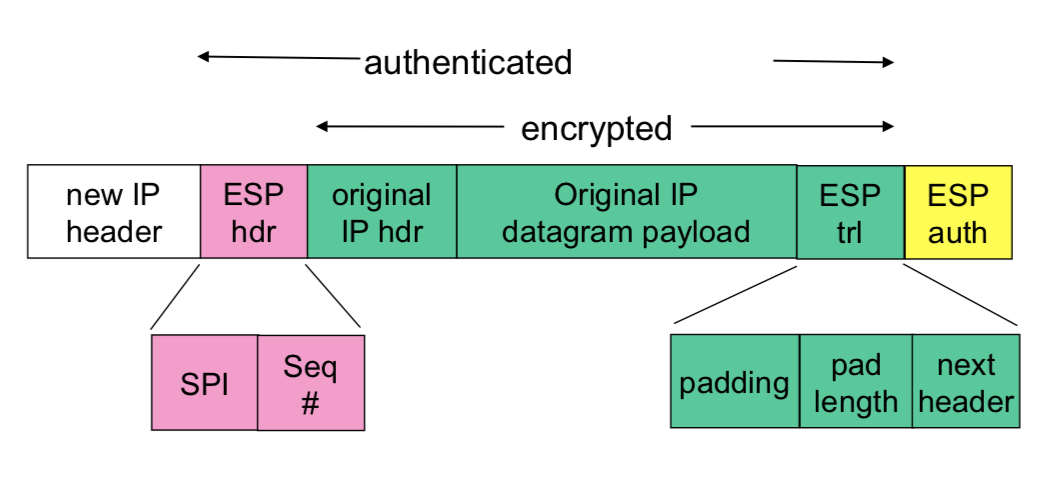
\includegraphics[width=\linewidth]{ipsec}
	\centering
	\caption{IPsec datagram (tunnel, ESP)}
\end{figure}
\begin{itemize}
	\item IKE message exchange for algorithms, secret keys, SPI numbers
\end{itemize}

\subsection{Firewalls}
\begin{description}
	\item[prevent DoS attacks:] SYN flooding, attacker establishes many bogus TCP connections, no resources left for ``real'' connections
	\item[prevent illegal modification/access of internal data:] e.g. attack replaces CIA's homepage with something else
	\item[allow only authorized access to inside network:] set of authenticated users/hosts
	\item[three types of firewalls:] stateless packet filters, stateful packet filters, application gateways
\end{description}
\subsubsection{Limitations of firewalls, gateways}
\begin{itemize}
	\item \textbf{IP spoofing:} router can't know if data ``really'' comes from claimed source
	\item if multiple applications need special treatment, each has own application gateway
	\item client software must know how to contact gateway (e.g. must set IP address of proxy in Web browser)
	\item filters often use all or nothing policy for UDP
	\item \textbf{tradeoff:} degree of communication with outside world, level of security
	\item many highly protected sites still suffer from attacks
\end{itemize}
\subsubsection{Intrusion detection systems}
\begin{itemize}
	\item packet filtering:
	\begin{itemize}
		\item operates on TCP/IP headers only
		\item no correlation check among sessions
	\end{itemize}
	\item \textbf{IDS:} Intrusion detection system
	\begin{description}
		\item[deep packet inspection:] look at packet contents (e.g. check character strings in packet against database of known virus, attack strings
		)
		\item[examine correlation] among multiple packets (port scanning, network mapping, DoS attack)
	\end{description}
\end{itemize}